\documentclass[12pt]{article}
\usepackage{graphicx}
\usepackage {color}
\usepackage{pdfpages}
\usepackage{float}
\usepackage{changebar}
\usepackage{enumitem,amssymb}
\renewcommand{\familydefault}{\sfdefault}
\usepackage[margin=1.2in]{geometry}
\usepackage{graphicx}
\usepackage{wrapfig}
\usepackage[super]{cite}
\usepackage{subcaption}
\usepackage[table]{xcolor}
\usepackage{amsmath}
\usepackage[sort, numbers]{natbib}
\usepackage{multirow}
\usepackage{tabularx}
\usepackage{siunitx}
\usepackage{matlab-prettifier}
\usepackage{wrapfig,lipsum,booktabs}
%%%%%%%%%%%%Defining the margins %%%%%%%%%%%%%%%%%%%%%
\textheight 9.in
\textwidth 6.5in
\topmargin -.5in
\oddsidemargin 0in
\setlength{\parskip}{\smallskipamount}

%%%%%%%%%%%%%%Specific Commands %%%%%%%%%%%%%%%%%%
\newcommand{\eg}{{\em e.g.,}}
\newcommand{\ie}{{\em i.e.,}}
\newcommand{\etc}{{\em etc.,}}
\newcommand{\etal}{{\em et al.}}
\newcommand{\degrees}{{$^{\circ}$}}
\newcommand{\fig}[1]{\textbf{Figure #1}}

%%%%%%%%%%%%%%%%%%%%%%%%%%%% Setting to control figure placement
% These determine the rules used to place floating objects like figures 
% They are only guides, but read the manual to see the effect of each.
\renewcommand{\topfraction}{.9}
\renewcommand{\bottomfraction}{.9}
\renewcommand{\textfraction}{.1}
\renewcommand{\familydefault}{\sfdefault} %setting the san serif font

%%%%%%%%%%%%%%%%%%%%%%%% Line spacing
% Use the following command for ``double'' spacing
%\setlength{\baselineskip}{1.2\baselineskip}
% and this one for an acceptable NIH spacing of 6lpi based on 11pt
%\setlength{\baselineskip}{.9\baselineskip}
% The baselineskip does not appear to work when we include a maketitle
% command in the main file.  Something there must set the line spacing
% If we use this next command, then things seem to work.
\renewcommand{\baselinestretch}{.9}

\setcounter{secnumdepth}{0} %make no numbers but have a table of contents


\begin{document}

\title{HW 4: Medical Imaging Systems}
\author{Jake Bergquist, u6010393 }
\maketitle

\section{Q1}
\noindent\textbf{a: } Attached is the sketch of the emission spectrum for the element in question. Using these K, L, and M binding energies we calculate a $K_\alpha = 22.0 keV$, a $K_\beta = 24.4 keV$, and $L_\alpha = 2.4 meV$. The $L_\alpha$ peak is filtered out by the $10 keV$ filter assumed in the problem statement. Thus with a $30 keV$ source we get the usual emission spectrum shape with a peak at the $K_\alpha$ and $K_\beta$ energies. Also shown in dotted lines is the shape of the emission curve without the filtering.

\noindent\textbf{b: } Attached is the sketch of the emission spectrum with additional filtering by the element. First of all we know that there will be a decreased emission due to the general blanket absorption of the element. Additionally the element will have sharp spikes in absorption at its K, L, and M binding energies. The absorption profile for this element is shown in the attached figure. The L and M shelves are below the 1$10keV$ filter and thus will have no effect but the K binding energy of $25 keV$ will cause a K shelf to be seen int he emission spectrum when filtered by this element, sharply filtering our energies at or above this energy. The dashed line shows the original emission.

\section{Q2}
\noindent\textbf{a: } 
For a given number of photons that enter a material, $N_{in}$, we know that the number of photons leaving that material, $N_{out}$, is given by Eq~\ref{eq3} below where $\mu$ is the mass attenuation coefficient of the material and $t$ is the thickness of the tissue.
 \begin{equation}
 N_{out} = N_{in}e^{-\mu t}
 \label{eq3}
 \end{equation}
\noindent Additionally we know that the intensity of the x-ray beam is given by $I = NE$ where $N$ is the number of photons and $E$ is the energy. Additionally we know that the number of photons, $N$, can be expressed as $N = A_{roi}\lambda$ where $A_{roi}$ is the area of the region of interest and $\lambda$ is the fluence of the source. Using these relationships and Eq~\ref{eq3} we can get an expression for each of our beam intensities. For $beam_2$ this is easy because here is only one mass attenuation coefficient and one tissue thickness thus:\\ $I_{beam2} = EA_{roi}\lambda e^{-\mu_{tissue}t_{tissue}}$\\ For $beam_1$ we have two tissues (tissue and vessel) and the two thicknesses. Thus our expression becomes \\$I_{beam1} =EA_{roi}\lambda e^{-\mu_{vessel}t_{vessel}}e^{-\mu_{tissue}(t_{tissue}-t_{vessel})}$\\

\noindent\textbf{b: }
The equation for $beam_2$ is unchanged with the contrast. The equation for $beam_1$ becomes:\\
$I_{beam1} =EA_{roi}\lambda e^{-\mu_{contrast}t_{vessel}}e^{-\mu_{tissue}(t_{tissue}-t_{vessel})}$\\

\noindent\textbf{c: }
Let us first consider the case with $beam_1$. We have $I_0^1$ which is the intensity of $beam_1$ without contrast and $I_c^1$ which is the intensity with contrast. If we divide one by the other, say $I_C^1$ by $I_0^1$ we see that most of the terms cancel out and we are left with two exponentials relating the attenuation coefficients of the vessel and the contrast as below:\\
$\frac{I_c^1}{I_0^1} = \frac{EA_{roi}\lambda e^{-\mu_{contrast}t_{vessel}}e^{-\mu\\
		_{tissue}(t_{tissue}-t_{vessel})}}{EA_{roi}\lambda e^{-\mu_{vessel}t_{vessel}}e^{-\mu_{tissue}(t_{tissue}-t_{vessel})}} = \frac{e^{-\mu_{contrast}t_{vessel}}}{e^{-\mu_{vessel}t_{vessel}}}$
Taking the natural log and rearranging we get the following:\\
$ln(I_c^1) - ln(I_0^1) = ln(e^{-\mu_{contrast}t_{vessel}}) - ln(e^{-\mu_{vessel}t_{vessel}}) = -\mu_{contrast}t_{vessel}+\mu_{vessel}t_{vessel}$\\
In this form we have a resulting subtraction intensity:\\
$I_s^1 = ln(I_c^1) - ln(I_0^1) = -\mu_{contrast}t_{vessel}+\mu_{vessel}t_{vessel}$.\\
Now lets look at $beam_2$ using the same notation with $I_0^2$ being before contrast and $I_c^2$ as after. When we apply the same method we see that all of the terms cancel and we are left with 1 on the right side of the equation:\\
$\frac{I_c^2}{I_0^2} = \frac{EA_{roi}\lambda e^{-\mu_{tissue}t_{tissue}}}{EA_{roi}\lambda e^{-\mu_{tissue}t_{tissue}}} = 1$\\
Again taking the natural log as before and rearranging we get our expression:\\
$I_s^2 = ln(I_c^2) - ln(I_0^2) = ln(1) = 0$\\
Thus for our final result we get an intensity that depends on the attenuation coefficients of the vessel and contrast when the beam passes through a vessel, and an intensity that is 0 everywhere there is not contrast. Thus we have removed the contribution of the tissue and have achieved our contrast intensities that highlight the areas where the contrast goes.


\section{Q3}
When there is no detector response we can use the geometry of our setup to construct a situation where we cal solve for $s$, the minimum spacing when the two circles just start to touch very easily. This is shown in the attached figure (Q3.a). However when we have a detector response as mentioned in the question this figure needs to be altered. The closest that the two edges of the circles on the detector can get is now not the point at which the two beams that make up these edges hit the detector, because every time a beam hits the detector the detector will respond with a circle with radius of $R_d$. Thus when the two circles are closest without overlapping is when the detector responses at the edges of these circles just barely meet. Thus we get a geometry as seen in the attached figure Q3.b. Here z denotes the distance from the pinhole to the source, d is the distance to the detector from the source,  is the spacing of the pinholes, $R_d$ is the detector response radius, and $R_s$ is the source radius. In this configuration we have two trapezoids. If our line $s$ was the midline of the larger trapezoid, finding its length would be easy due to the midpoint theory. However we do not assume that the distance between the pinhole and the source is equal to the pinhole and the detector. Thus we must look another way. If we re draw this geometry in a bit more detail as in Q3.c we see that we can solve for the length of $s = 2R_d+2x$. In this figure the triangle formed by $(d-z)$, $x$, and the outter edge is simmilar tot he one formed by $a$, $d$, and the outer edge. We also know that $a = R_s-R_d$. Thus using this simmilar triangle we can solve for $x$ as follows:\\
$\frac{a}{x} = \frac{d}{d-z}$\\
$x = \frac{a(d-z)}{d} = \frac{R_s-R_d)(d-z)}{d}$\\
Now with a value for $x$ we can plug this into our equation for $s$ to get:\\
$s = 2R_d +2x = 2R_d + 2(\frac{(R_s-R_d)(d-z)}{d})$\\
This is the minimum $s$ where the two pinholes an be resolved on the detector, or rather that minim s is given byt he above expression plus $\epsilon$ where $\epsilon$ is some very small value. This is because at the point defined above the two circles have just begun to touch on the detector and thus would just barely begin to be unresolvable from each other. Thus the true minimum $s$ is just slightly larger than this. If the ratio of $R_s$ to $R_d$ is 1 then the resolution is independent of $z$ because the second term with the $(R_s-R_d) => 0$ thus our resolution is only dependent on $R_d$ in that case.

In the geometry of the case above we considered that the detector response radius was smaller than the source radius ($R_d <= R_s$). We need to check to make sure how things might change if we reverse this assumption. If we redraw Q3.c such that $R_s < R_d$ we get Q3.d. Again there are many clever ways we can solve for s in this scenario but lets follow the same approach as before such that in Q3.d, $s = 2R_s + 2x$. Already we have something different. If we carry though like we did before we get the following:\\
$a = R_d - R_s\\
\frac{a}{X} = \frac{d}{z}\\
x = \frac{az}{d} = \frac{(R_d-R_s)z}{d}\\
s = 2R_s + 2(\frac{(R_d-R_s)z}{d})\\$
However if we look closely, yes in this scenario our determination of the minimum resolution, $s$, has changed, it is still true that having the ratio of $R_s$ and $R_d$ be one results in a determination that is not dependent on $z$. In this case where this ratio is true then $R_s$ = $R_d$, thus the resolution is $s = 2R_s = 2R_d$, no matter what the geometry is. This becomes appearant when we draw it as seen in Q3.e. (All figures for this problem are attached at the end.)


\section{Q4}
First we want to figure out what the exposure is at the lungs that would lead to a dose of 10 mrems = 0.01R. To do so we can use the relationship shown in Eq~\ref{eq1} that relates Dose ($D$) to Exposure ($X$).
\begin{equation}
D = \frac{0.873(\frac{\mu}{\rho})_{tissue}}{(\frac{\mu}{\rho})_{air}}X
\label{eq1}
\end{equation}
\noindent We can then check the National Institute of Standards and Technology (NIST) which keeps a database for the mass attenuation coefficients of various materials at various energies. At $50keV = 5\cdot10^{-2}MeV$ we find that dry air near sea level (which we assume to be our case) has a mass attenuation coefficient of $(\frac{\mu}{\rho})_{air} = 0.2080\frac{cm^2}{g}$. For lung tissue we find that at $50keV$ we get a mass attenuation of $(\frac{\mu}{\rho})_{lung} = 0.2270\frac{cm^2}{g}$. Substituting these into [\ref{eq1}] and solving for X we get an exposure of $X = \frac{D(\frac{\mu}{\rho})_{air}}{0.873(\frac{\mu}{\rho})_{lung} } = \frac{0.01 R \cdot 0.2080\frac{cm^2}{g}}{0.873\cdot 0.2270\frac{cm^2}{g}} = 0.0105 R$. 

\noindent Now we know what the exposure needs to be at the location of the lungs. Using this and our knowledge of what the exposure is 1cm from the source (10R) we can find out how far from the source we need to be in order to get  our desired exposure. To do so we use the inverse square law to determine what the distance to get this exposure is. Eq~\ref{eq2} shows us this relationship. By plugging in $1cm$ for $D_1$, $10R$ for $X_1$, and $0.0105R$ for $X_2$ then solving for $D_2$ we get our desired distance.
\begin{equation}
\frac{D_1^2}{D_2^2} = \frac{X_2}{X_1}
\label{eq2}
\end{equation}
\noindent $D_2 = \sqrt{\frac{D_1^2X_1}{X_2}} = \sqrt{\frac{1cm^2\cdot 10R}{0.0105R}} = 30.9 cm$ We can rework this entire formulation, instead solving for the Dose delivered at 1 cm then using the inverse square to calculate at what distance this dose falls off to the desired 10 mrem, and doing so yields the same answer of 30.9 cm. Thus to be safe I would recommend placing the lungs of the patient at least 31 cm from the source. 
\section{Q5}
\noindent\textbf{a: } The formula for contrast is $c = \frac{\Delta I}{\overline{I}} \approxeq \frac{|I_b - I_{roi}}{I_b}$. In our case for the first part this is easy.The intensity of the region of interest is 0.2, and the background intensity is 1. Thus the contrast is $\frac{|1 - 0.2|}{1} = 0.8$.

\noindent\textbf{b\&c: }
For this section I used a matlab script to generate the images ar a range of lambda values ([10,5,2,1,0.8,0.6,0.4,0.3,0.2,0.1]) and the given range of intensities. I then used a script to display the images to the observer and prompt them if they could see the circle. The image was displayed on a full screen figure window. Observers were instructed to mark if they were or were not able to distinctly see one circle, and not to spend too long looking for them. 

\textbf{Note:} For each of the figures shown below, printing these images onto paper does not show the subtle differences between them well. In fact most of the images look indistinguishable and the circes can only be resolved on a computer screen. The observers were tested on computer screens where the differences between these images was more clear. At the end of the report before the hand drawn figures are full page sized versions of figures 1 2 and 3 to try to display the differences between them but this still does not print well. The pdf version shows these changes and highlights the difficulties in displaying figures and data in printed medium. I will provide the pdf upon request so that the images can be viewed as they were presented to the observers.

The results for observer 1 are shown in Table~\ref{Tab1} and Figure~\ref{Fig:obs1Img}. Observer 1 could not detect any circle for the final intensity images (Intensity 0.8) even at a fluence of 10. 
\begin{table}[H]
	\caption{Observer 1 Response: For each intensity the minimum lambda at which the circle was detected is shown as well as the contrast and SNR at that lambda value for that image.}
	\begin{tabular}{|l|l|l|l|}
		\hline
		Intensity & Min Lambda & Contrast & SNR  \\ \hline
		0.2       & 0.2        & 0.81     & 3.86 \\ \hline
		0.4       & 1          & 0.64     & 6.82 \\ \hline
		0.6       & 2          & 0.40     & 6.00 \\ \hline
		0.8       & n/a        & n/a      & n/a  \\ \hline
		
	\end{tabular}
\label{Tab1}
\end{table}

\begin{figure}[H]

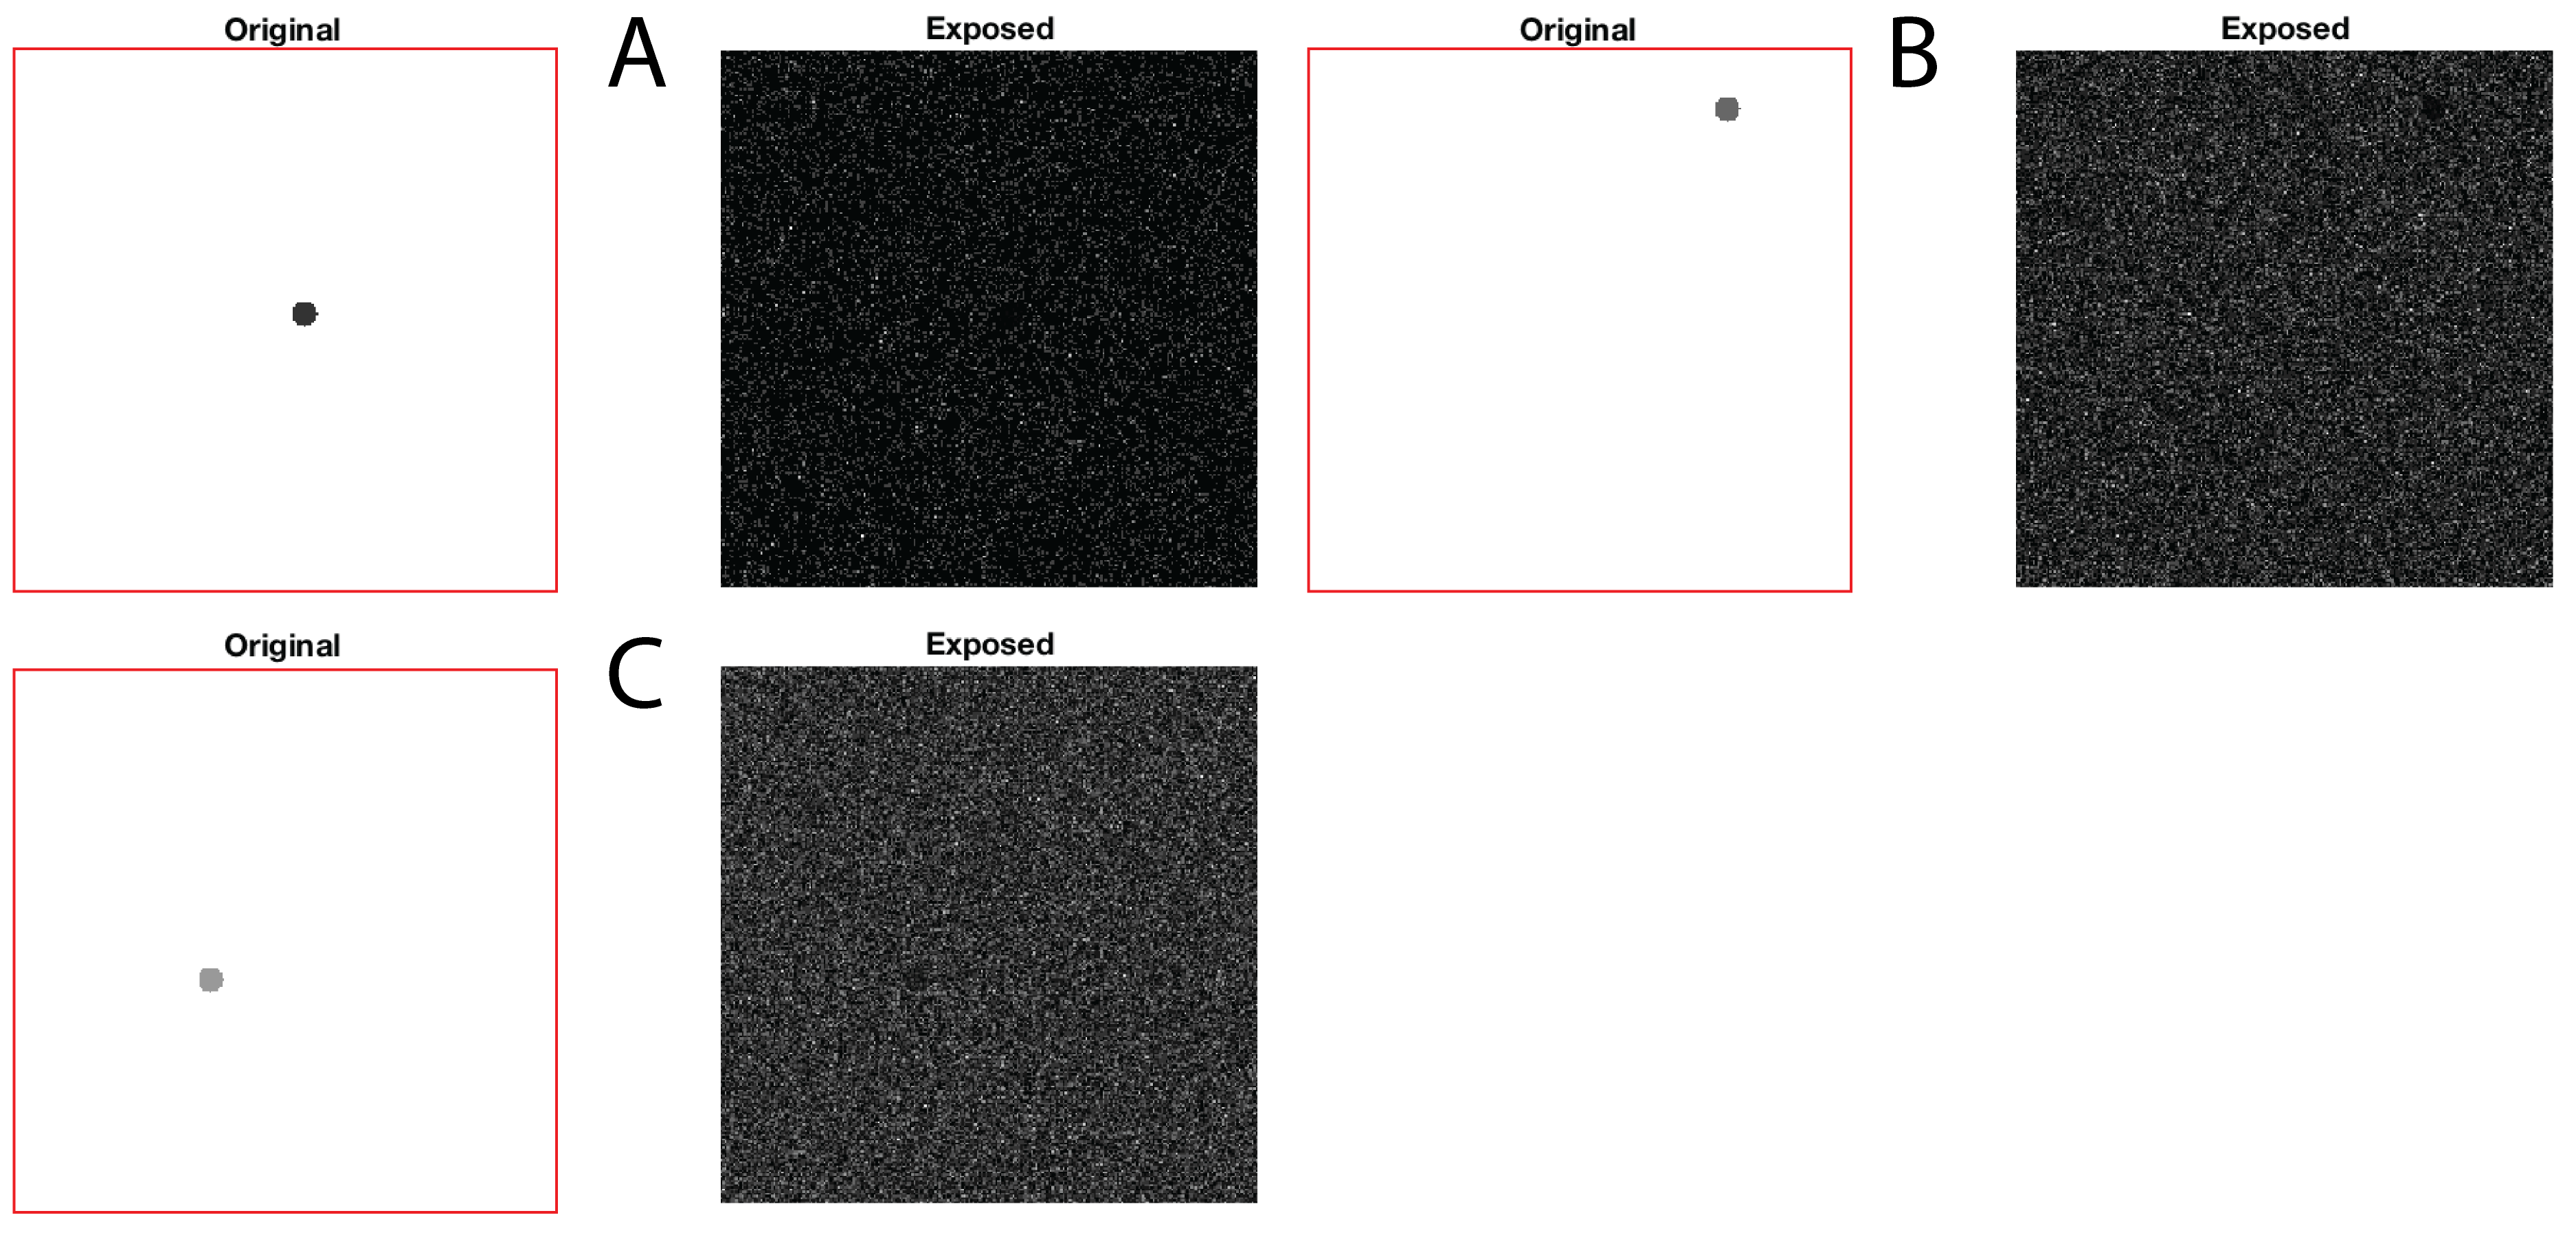
\includegraphics[width=\textwidth]{Figures/Obs1_fig.png}
\caption{Observer 1 minimum Lambda images: The original and exposed images for each intensity corresponding to the minimum lambda value at which the observer was able to detect a circle. A) the images for intensity of 0.2, lambda 0.2, B) intensity 0.4, lambda 1, D) intensity 0.6, lambda 2. This observer could not detect a circle at intensity 0.8 for any lambda value used.}
\label{Fig:obs1Img}
\end{figure}

The results for observer 2 are shown in Table~\ref{Tab2} and Figure~\ref{Fig:obs2Img}. Observer 1 followed observer 2 for the most part however observer 2 was able to detect a circle at the 0.8 intensity albeit only for the lambda value of 10. 

\begin{table}[H]
	\caption{Observer 2 Response: For each intensity the minimum lambda at which the circle was detected is shown as well as the contrast and SNR at that lambda value for that image.}
	\begin{tabular}{|l|l|l|l|}
		\hline
		Intensity & Min Lambda & Contrast & SNR  \\ \hline
		0.2       & 0.2        & 0.81     & 3.86 \\ \hline
		0.4       & 1          & 0.64     & 6.82 \\ \hline
		0.6       & 2          & 0.40     & 6.00 \\ \hline
		0.8       & 10         & 0.18     & 6.10 \\ \hline
	\end{tabular}
\label{Tab2}
\end{table}

\begin{figure}[H]
	
	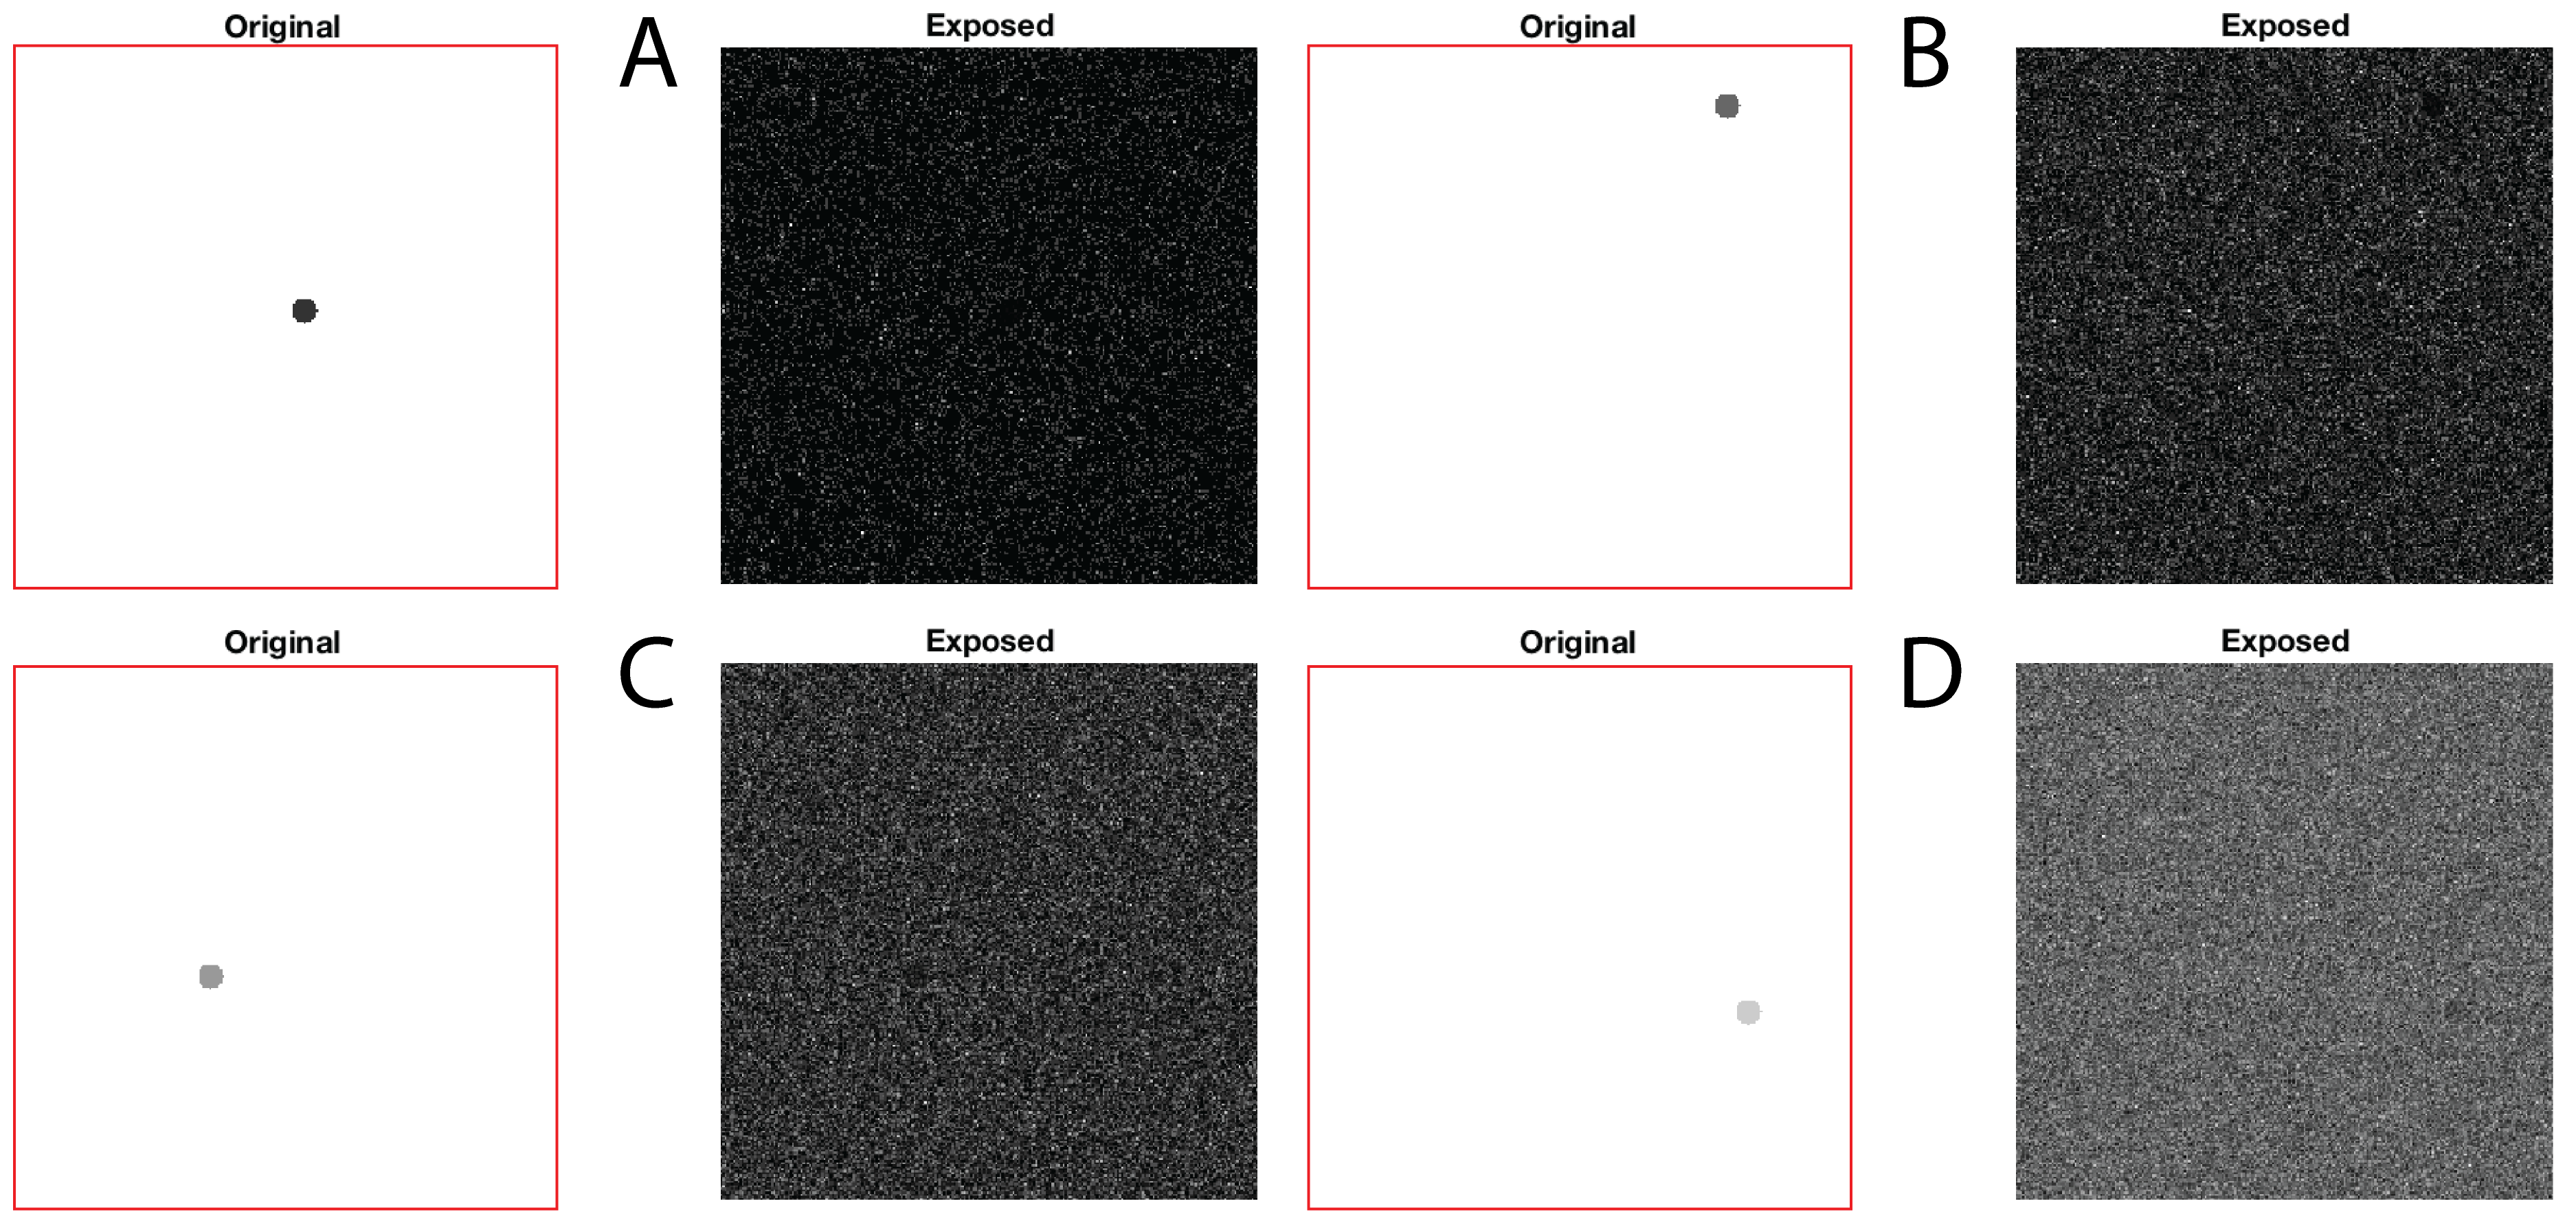
\includegraphics[width=\textwidth]{Figures/Obs2_fig.png}
	\caption{Observer 2 minimum Lambda images: The original and exposed images for each intensity corresponding to the minimum lambda value at which the observer was able to detect a circle. A) the images for intensity of 0.2, lambda 0.2, B) intensity 0.4, lambda 1, D) intensity 0.6, lambda 2. D) intensity 0.8, lambda 10}
	\label{Fig:obs2Img}
\end{figure}

The results for observer 3 are shown in Table~\ref{Tab3} and Figure~\ref{Fig:obs3Img}. Observer 3 Deviated fromt eh previous observers for the first and second intensities, and fell in line with observer two for the third and fourth intensities.

\begin{table}[H]
	\caption{Observer 3 Response: For each intensity the minimum lambda at which the circle was detected is shown as well as the contrast and SNR at that lambda value for that image.}
	\begin{tabular}{|l|l|l|l|}
		\hline
		Intensity & Min Lambda & Contrast & SNR  \\ \hline
		0.2       & 0.6        & 0.81     & 6.67 \\ \hline
		0.4       & 0.8        & 0.60     & 5.71 \\ \hline
		0.6       & 2          & 0.40     & 6.00 \\ \hline
		0.8       & 10         & 0.18     & 6.10 \\ \hline
	\end{tabular}
\label{Tab3}
\end{table}

\begin{figure}[H]
	
	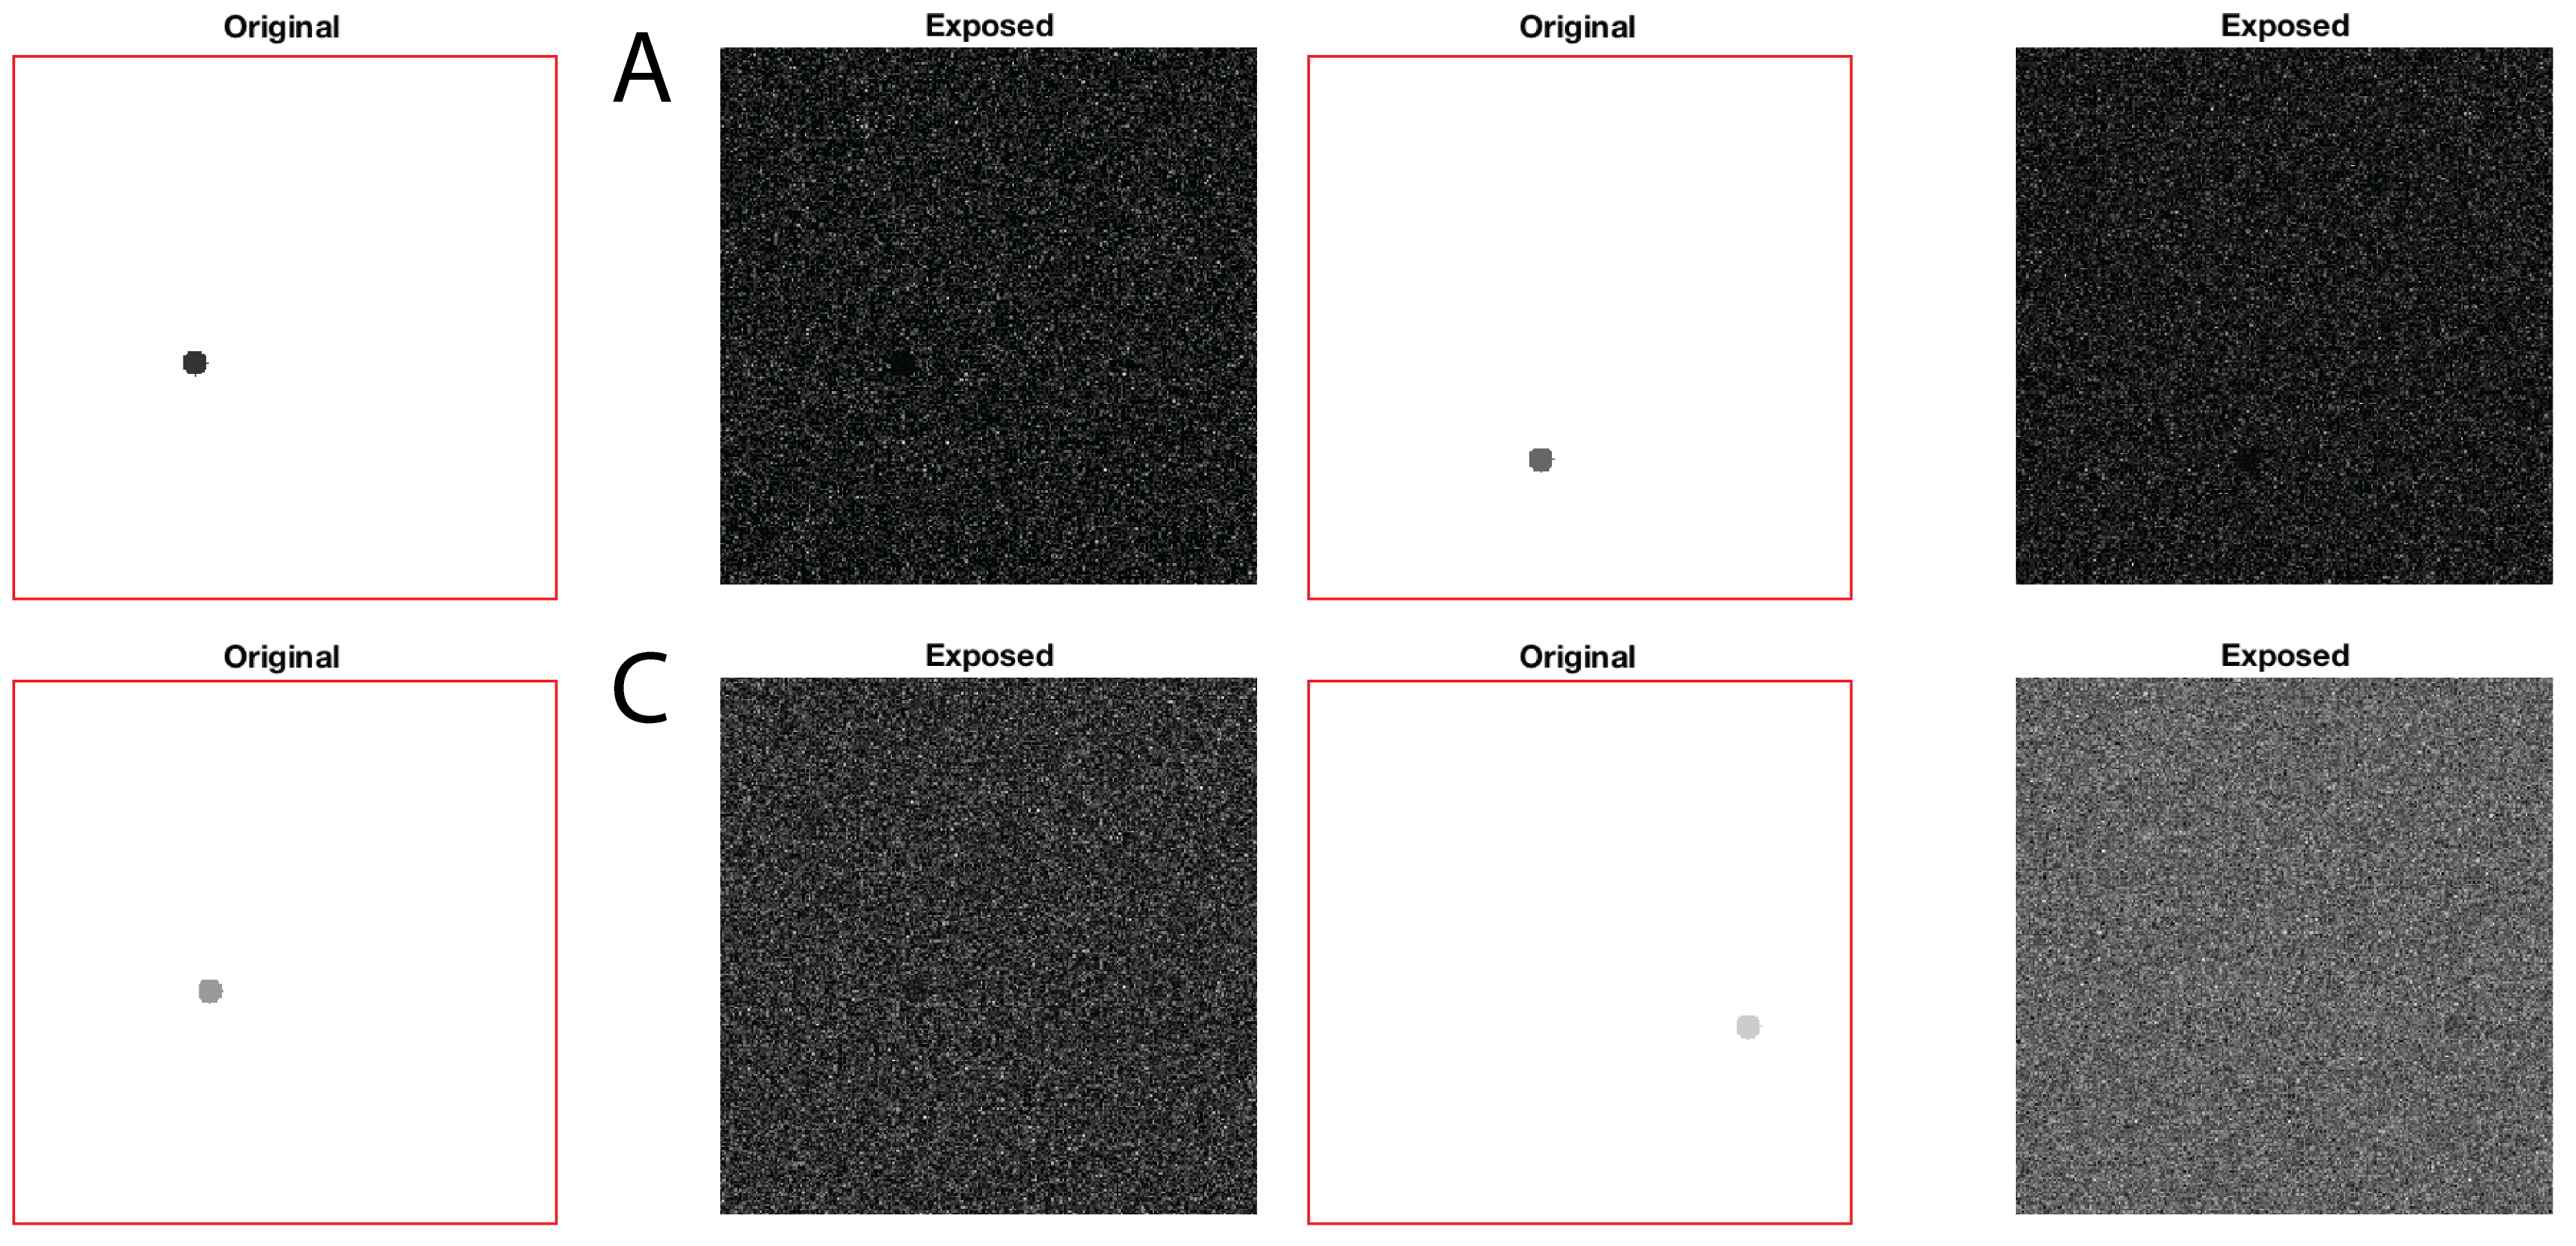
\includegraphics[width=\textwidth]{Figures/Obs3_fig.png}
	\caption{Observer 3 minimum Lambda images: The original and exposed images for each intensity corresponding to the minimum lambda value at which the observer was able to detect a circle. A) the images for intensity of 0.2, lambda 0.6, B) intensity 0.4, lambda 0.8, D) intensity 2, lambda 2. D) intensity 0.8, lambda 10}
	\label{Fig:obs3Img}
\end{figure}

Summarizing all of these numbers we see in Figure~\ref{Fig:lambdas} that as the intensity increased so too did the minimum lambda at which the observers could detect the circle. However, the contrast and SNR of the images at which the observers could barely detect the circle (with the minimum lambda for each intensity) have relatively uniform value as seen in Figure~\ref{Fig:Contrast}~and~\ref{Fig:SNR}. This suggests that the ability to see the circle is a function of the SNR and contrast more directly than it is of the lambda value. However all of these quantities are related. Below the figures is the MATLAB code used to generate the images and test the users

\begin{figure}[H]
	\centering
	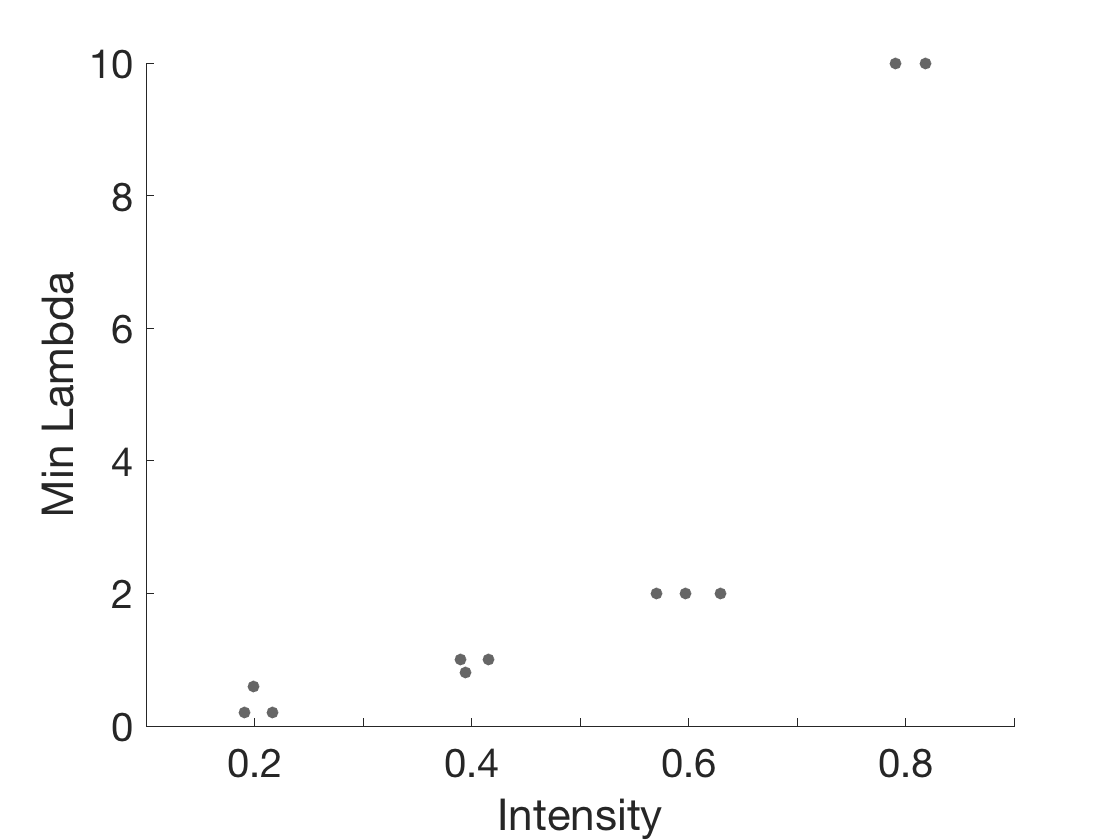
\includegraphics[width=0.8\textwidth]{Figures/Lambda.png}
	\caption{Minimum lambda per intensity}
	\label{Fig:lambdas}
\end{figure}

\begin{figure}[H]
	\centering
	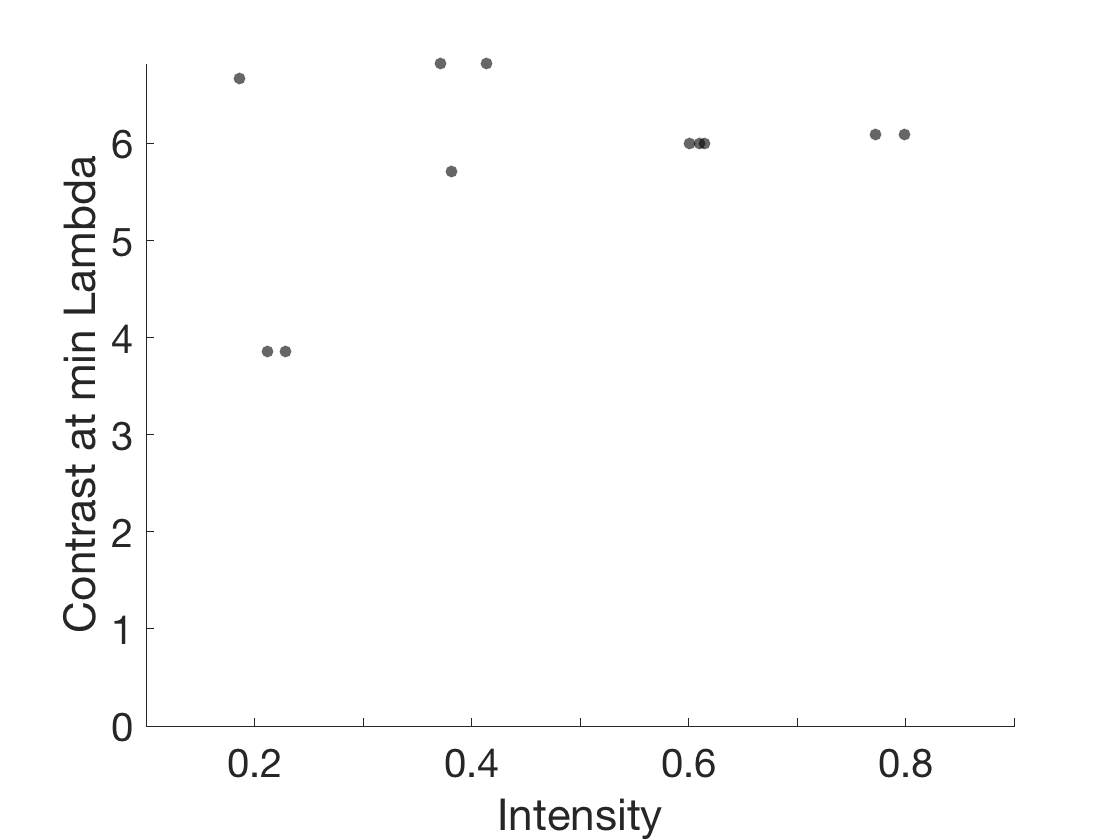
\includegraphics[width=0.8\textwidth]{Figures/Contrasts.png}
	\caption{Contrast at minimum lambda per intensity}
	\label{Fig:Contrast}
\end{figure}


\begin{figure}[H]
	\centering
	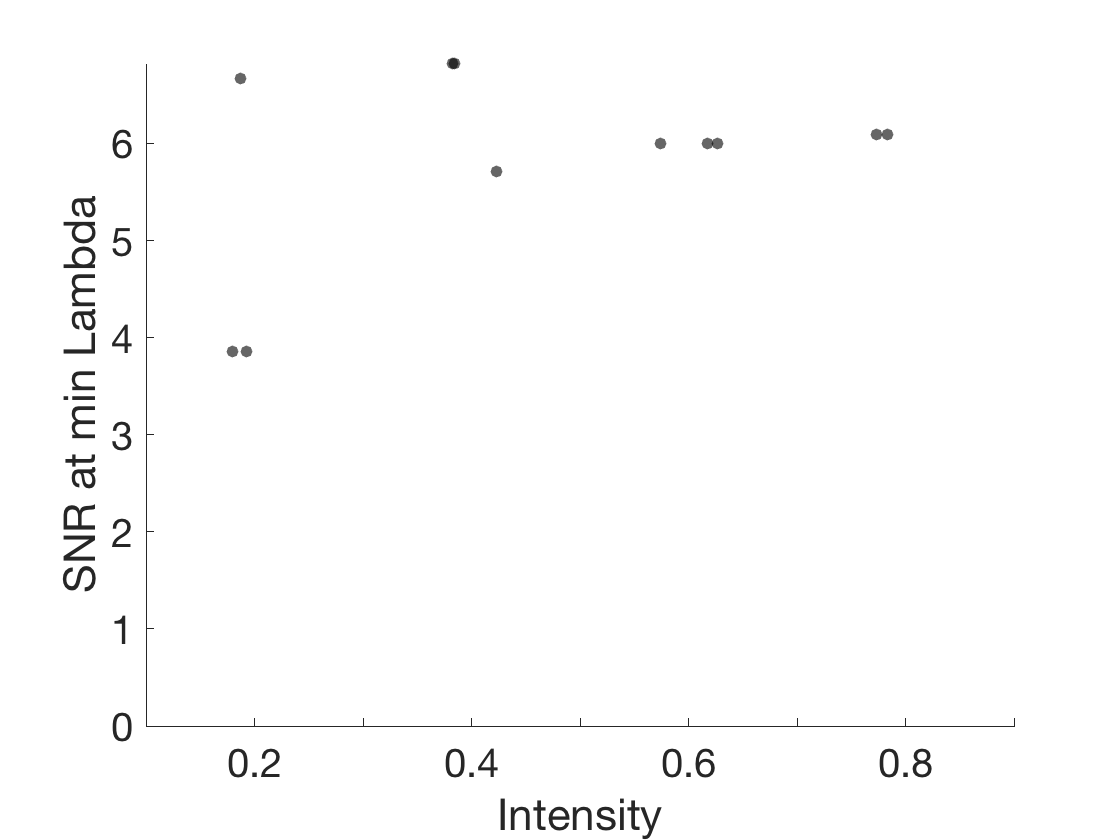
\includegraphics[width=0.8\textwidth]{Figures/SNRs.png}
	\caption{SNR at minimum lambda per intensity}
	\label{Fig:SNR}
\end{figure}

\begin{lstlisting}[style=Matlab-editor]
%%

lambdaVals = [10,5,2,1,0.8,0.6,0.4,0.3,0.2,0.1];
intensities = [0.2,0.4,0.6,0.8];

%Generate the images for me to look at
for ind1 = 1:length(intensities)
for ind2 = 1:length(lambdaVals)
currentIndex = length(lambdaVals)*(ind1-1) + ind2;
fprintf(sprintf('index: %d\n',currentIndex))
%Generate new image for each lambda value
images(currentIndex).original = gen_im(6,intensities(ind1));
dist = poissrnd(lambdaVals(ind2),256,256);
dist = dist/max(dist(:));
images(currentIndex).exposed = dist.*images(currentIndex).original;
%Display to check that it was done right
figure(currentIndex); clf();
subplot(211);
imshow(images(currentIndex).original);
title(sprintf('Original for Labmda %d, intensity %d',lambdaVals(ind2),intensities(ind1)))
subplot(212);
imshow(images(currentIndex).exposed);
title(sprintf('Exposed for Labmda %d, intensity %d',lambdaVals(ind2),intensities(ind1)))
images(currentIndex).lambdaVal = lambdaVals(ind2);
images(currentIndex).intensity = intensities(ind1);
end
end
%Calculate contrast and SNR of each image
aROI = pi*6^2;%r = 6
for im = 1:length(images)

circleInds = find(images(im).original <1);
Iroi = mean(images(im).exposed(circleInds));
Ib = mean(images(im).exposed(setdiff([1:length(images(im).exposed(:))],circleInds)));
images(im).contrast = abs(Ib-Iroi)/Ib;
images(im).SNR = images(im).contrast * sqrt(1*images(im).lambdaVal*aROI);

end


save('images.mat','images')
%%

%Display the images for my user to see and evaluate
circleSeen = zeros(length(intensities),length(lambdaVals));
for ind1 = 1:length(intensities)
for ind2 = 1:length(lambdaVals)
currPosition = get(figure(1),'position');
currentIndex = length(lambdaVals)*(ind1-1) + ind2;
figure(1);
imshow(images(currentIndex).exposed);
title('Do you see a disntict circle?')
set(figure(1),'position',currPosition);
in = input('Do you see a circle in this image? 1:y 0:n ');
circleSeen(ind1,ind2) = in;
end
end
%%
save('observerResponse.mat','circleSeen')
\end{lstlisting}

\end{document}



\begin{figure}[H]
	\centering
	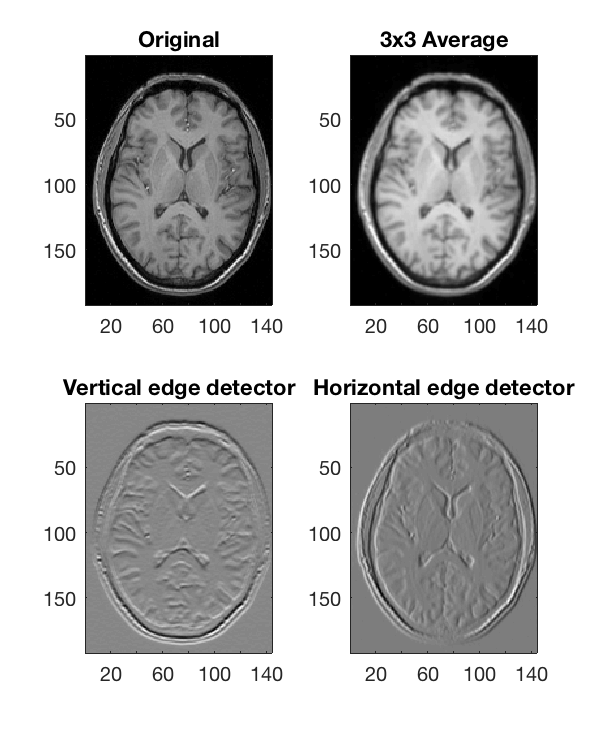
\includegraphics[width=\textwidth]{Figures/convs.png}
	\caption{}
	\label{Fig:conv}
\end{figure}

\begin{lstlisting}[style=Matlab-editor]

\end{lstlisting}




